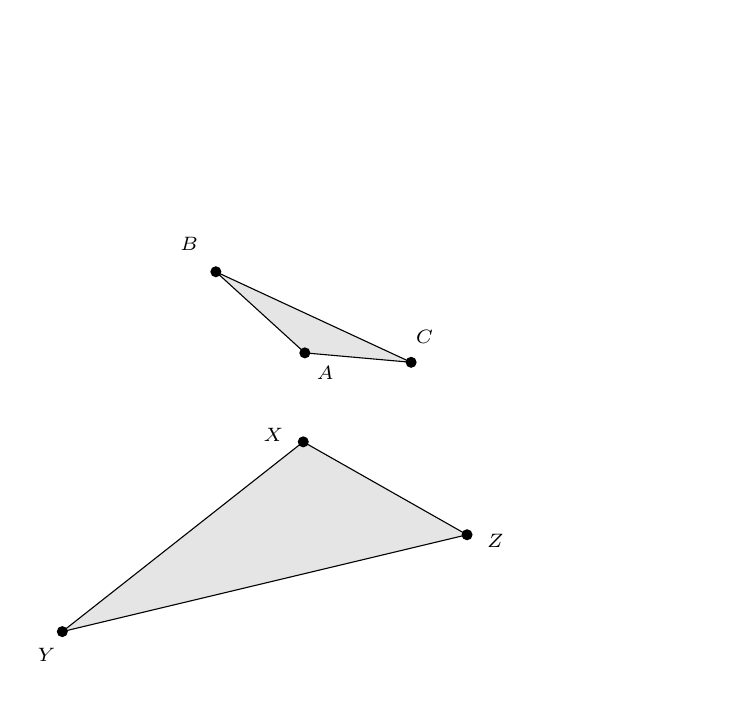
\begin{tikzpicture}[scale = 1]
    \clip(-5.5,-1.15) rectangle (3.12,7.27);
    \fill[fill=black,fill opacity=0.1] (-3.11,4.17) -- (-1.98,3.14) -- (-0.63,3.02) -- cycle;
    \fill[fill=black,fill opacity=0.1] (-5.06,-0.4) -- (-2,2.01) -- (0.08,0.83) -- cycle;
    \draw (-3.11,4.17)-- (-1.98,3.14);
    \draw (-1.98,3.14)-- (-0.63,3.02);
    \draw (-0.63,3.02)-- (-3.11,4.17);
    \draw (-5.06,-0.4)-- (-2,2.01);
    \draw (-2,2.01)-- (0.08,0.83);
    \draw (0.08,0.83)-- (-5.06,-0.4);
    \begin{scriptsize}
        \fill [color=black] (-1.98,3.14) circle (2.0pt);
        \draw[color=black] (-1.72,2.88) node {$A$};
        \fill [color=black] (-3.11,4.17) circle (2.0pt);
        \draw[color=black] (-3.45,4.52) node {$B$};
        \fill [color=black] (-0.63,3.02) circle (2.0pt);
        \draw[color=black] (-0.46,3.34) node {$C$};
        \fill [color=black] (-2,2.01) circle (2.0pt);
        \draw[color=black] (-2.38,2.1) node {$X$};
        \fill [color=black] (-5.06,-0.4) circle (2.0pt);
        \draw[color=black] (-5.26,-0.7) node {$Y$};
        \fill [color=black] (0.08,0.83) circle (2.0pt);
        \draw[color=black] (0.44,0.75) node {$Z$};
    \end{scriptsize}
\end{tikzpicture}